Extensive exploration and experiments have been done to validate our approach as well as to evaluate 
its performance under various workload patterns. This section covers our testbed setup, experimental 
methodologies, performance tuning, results, and analysis. 

\subsection{Testbed setup}
The experiments are conducted in two phases. In the first phase, only CPU is over-committed 
to isolate and evaluate its effects. 
In this phase, we use a cluster of 18 nodes (including 1 login node, 1 management node, and 16 compute nodes, see Figure~\ref{fig:architecture}) to mimic a realistic HPC computing environment. Each node has dual 10-core Intel Xeon E5-2660 processor, 128 GB DDR4 memory, and 1 Gb Ethernet network. 
The hypervisor used is VMware ESXi 6.5, OS is CentOS 7.2, and HPC resource manager is TORQUE 6.1 with its default job scheduler. We use compute-intensive benchmarks from PolyBench/C 3.1 and BioPerf~\cite{1526013}. 
In the second phase, we evaluate the full-fledged solution with both CPU and memory over-commitment on another testbed with large memory capacity for memory-intensive workloads. The second cluster has 1 login, 1 management, and 8 compute nodes. Each node has dual 16-core Intel Xeon Gold 6130 processor, 768 GB DDR4 memory, and 2x 10 Gb Ethernet cards. 
The hypervisor used is VMware ESXi 6.7, OS is CentOS 7.6, and resource manager is TORQUE 6.1 with its default job scheduler. In addition to PolyBench/C and BioPerf, we add memory-intensive benchmarks from HPCC~\cite{dongarra2004introduction}. The hardware details and software stack are summarized in Table~\ref{tbl:hardware} and \ref{tbl:software}, respectively. 

\begin{table}[!h]\small
  \caption{Hardware details.}
  \centering
    \begin{tabular}{|l|c|c|}
    \hline
     & Phase 1 & Phase 2 \\
    \hline
    Server & Dell PowerEdge C6320 & Dell PowerEdge R740 \\ 
    \hline
    \multirow{2}{*}{CPU} & 2X 10-core Intel Xeon  & 2X 16-core Intel Xeon  \\
                               &  E5-2660 v3@ 2 .6GHz & Gold 6130@2.1GHz \\
    \hline
    Memory & 128GB DDR4 & 768 GB DDR4 \\
    \hline
    Network & 1Gb Ethernet & 2X 10 Gb Ethernet \\
    \hline
    \end{tabular}
  \label{tbl:hardware}
\end{table}

\begin{table}[!h]\small
  \caption{Software stack.}
  \centering
    \begin{tabular}{|l|c|c|}
    \hline
     & Phase 1 & Phase 2 \\
    \hline
    Hypervisor & ESXi 6.5 & ESXi 6.7 \\
    \hline
    Native/guest  & CentOS 7.2 & CentOS 7.6 \\
         OS       & (3.10.0-327) & (3.10.0-957) \\
    \hline
    Job scheduler & TORQUE 6.1 & TORQUE 6.1 \\
    \hline
    MPI & N/A & OpenMPI 3.0.3 \\
    \hline
    \multirow{2}{*}{Benchmarks} & PolyBench/C 3.1,  &  PolyBench/C 3.1,  \\
                                & BioPerf & BioPerf, HPCC \\  
    \hline
    \end{tabular}
  \label{tbl:software}
\end{table}

In addition, we also tune the BIOS settings as listed in Table~\ref{tbl:bios}.
%following VMware's best practice 
%guide in order to achieve the optimal performance~\cite{hpc2018best}. These tunings involve 
%power profile, HyperThreading, etc., and are applied in both phases. The details are listed in Table~\ref{tbl:bios}.
%Note that the same settings are applied in phase 1 and phase 2. 

\begin{table}[!h]\small
  \caption{BIOS settings}
  \centering
    \begin{tabular}{|l|c|}
    \hline
    System profile & Performance per watt (OS) \\
    \hline
    Logical Processor  & Enabled (2 threads per core) \\
    \hline
    Virtualization Technology & Enabled \\
    \hline
    Turbo Boost Technology & Enabled \\
    \hline
    Memory Interleaving & Disabled \\
    \hline
    \end{tabular}
  \label{tbl:bios}
\end{table}


\subsection{CPU over-commitment}
For performance comparison, each node is installed with two execution environments on two separate boot disks, that is, a native OS and an ESXi hypervisor. With the hypervisor, we further define three execution scenarios: 1) one VC; 2) two VCs; 3) four VCs. The latter two scenarios represent 2X and 4X CPU over-commitment, respectively. 3248 jobs are randomly sampled from PolyBench and BioPerf to construct a job stream. 
When comparing performance, we've arranged to maintain (roughly) the same job sequence 
regardless of the the number of clusters. Comparison of the wall clock execution time is shown in Figure~\ref{fig:cpu_exe_time}.

\begin{figure}[!t]
   \begin{center}
       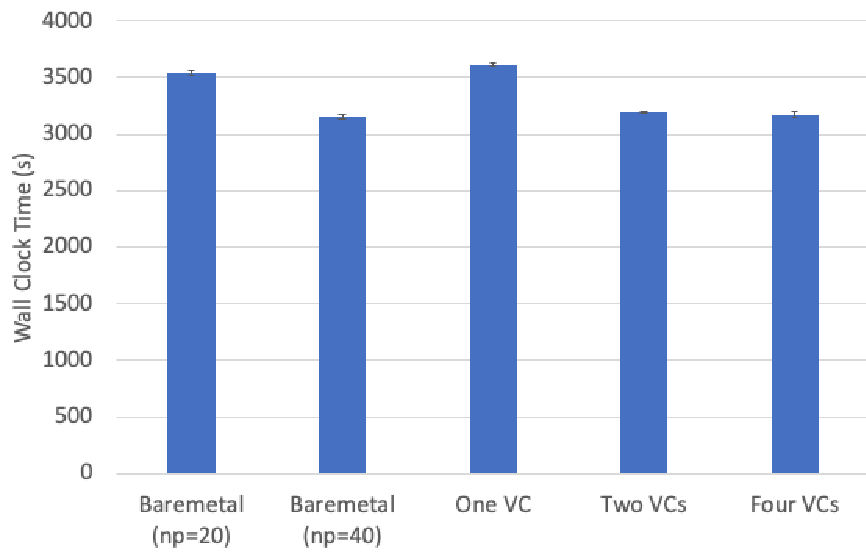
\includegraphics[width=0.8\columnwidth]{Figures/cpu_exe_time.pdf}
   \end{center}
   \caption{Comparison of wall clock time for a job stream between bare-metal and virtual clusters with different CPU over-commitment ratios. Results are average of three runs.}
   \label{fig:cpu_exe_time}
 \end{figure}

Because each node has 20 cores, in the first experiment we configure each TORQUE worker with 20 job slots. As reflected in Figure~\ref{fig:cpu_exe_time}, the execution time with one VC is very close to that of bare-metal, with only a 2.2 percent overhead. Furthermore, when multiple VCs are running, the execution time is surprisingly shorter. %, implying an improved throughput despite the virtualization overhead. 
Through careful analysis, we identify the reason to be increased CPU utilization when more jobs are concurrently scheduled to execute, taking advantage of HyperThreading (HT). This has been verified by modifying each TORQUE worker in bare-metal to use 40 job slots, after which the throughput is improved to the same level as the over-committed virtual environment. Note that HT is only advised to turn on in a trusted environment, such as when side-channel attack is not a concern. 
%This can be seen in the second column of Figure~\ref{fig:cpu_exe_time}.

Besides execution time, another performance metric that we monitor is the CPU utilization. On ESXi, we use esxtop running on each compute node to sample CPU utilization of all VMs at 5-second intervals, and the timeline view for one, two, and four VCs is shown in Figure~\ref{fig:cpu_utilizations}. 
Note that, ignoring HyperThreading and Turbo, the theoretical maximum utilization across the 16 20-core nodes can 
be calculated as 16 * 20 * 100\% = 32,000\%. Apparently, Figure~\ref{fig:cpu_utilizations} reveals that HyperThreading and Turbo 
are able to improve CPU utilization beyond above maximum value. 

%With two and four VCs, the decreasing trend at the end in Figure~\ref{fig:cpu_utilizations} is due to job completion. 
Clearly, CPU utilization in Figure~\ref{fig:cpu_utilizations} is consistent with the job execution time in Figure~\ref{fig:cpu_exe_time}. For example, the lowest CPU utilization case--one VC--matches the longest job execution time. 
The higher CPU utilization achieved by two and four VCs is due to resource consolidation brought about by virtualization. That is, when multiple VCs share a physical cluster, the ESXi CPU scheduler has more jobs to schedule and is therefore able to make better scheduling decisions by taking advantage of HyperThreading and eliminating idle cycles. 
With that, it's not surprising to see that the decreasing CPU utilization with two and four VCs at the end is due to faster job completion. 
At the same time, improved utilization also comes with better consistency, where the utilization with two and four VCs is much smoother than that in the single-cluster case.

\begin{figure}[!t]
   \begin{center}
       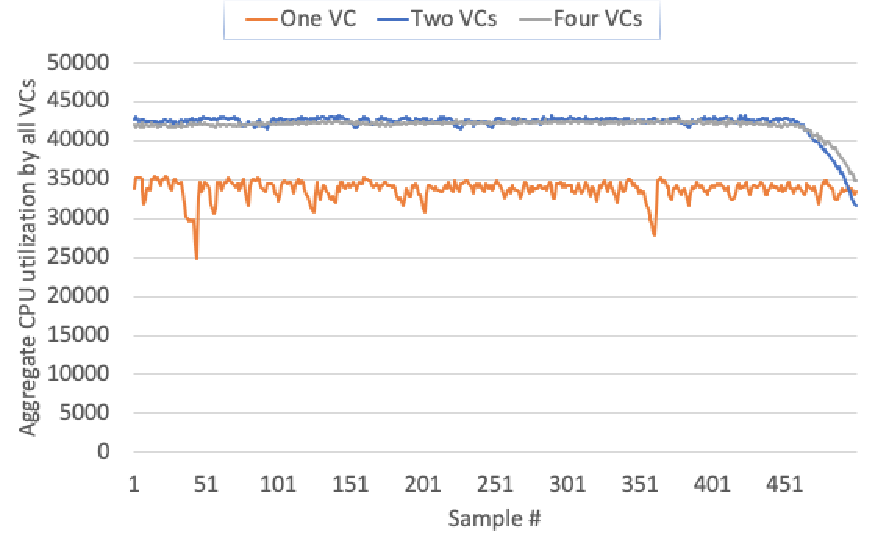
\includegraphics[width=0.8\columnwidth]{Figures/cpu_utilizations.pdf}
   \end{center}
   \caption{Aggregate CPU utilization across 16 compute nodes at 5-second intervals.}
   \label{fig:cpu_utilizations}
   %\vspace{-0.2in}
 \end{figure}

 In a production cloud environment, an important principle is fairness when multiple tenants share the computing resources. We further examine the per-cluster CPU utilization in the multiple-cluster, CPU over-committed cases.  The cases of four VCs are depicted in Figure~\ref{fig:per_cluster_utilization}. As we would expect, when giving the same shares to all the VMs the ESXi CPU scheduler effectively maintains fairness so that each VC gets the same amount of CPU resources. The case of two VCs is the same thus not shown here. 

\begin{figure}[!t]
   \begin{center}
       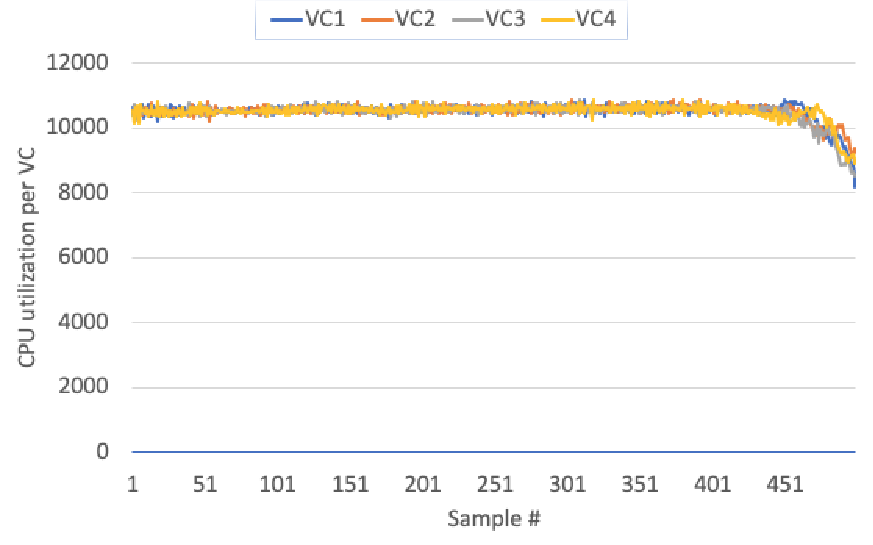
\includegraphics[width=0.8\columnwidth]{Figures/per_cluster_utilization_4.pdf}
   \end{center}
   \caption{Plot of CPU utilization per VC at 5-second intervals for fairness check.}
   \label{fig:per_cluster_utilization}
   %\vspace{-0.2in}
\end{figure}
% \begin{figure}[!t]
%    \begin{center}
%       \begin{subfigure}[b]{0.35\textwidth}
%          %\centering
%          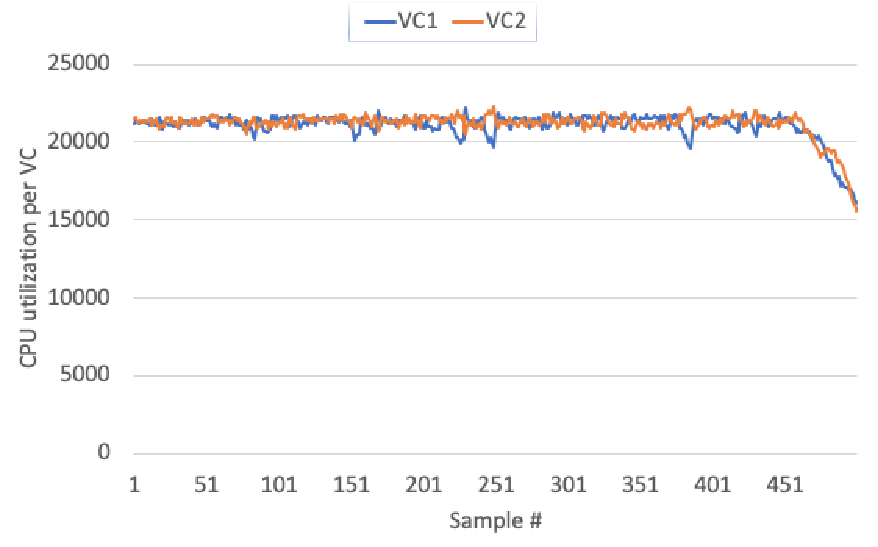
\includegraphics[width=\textwidth]{Figures/per_cluster_utilization_2.pdf}
%          \caption{Running two VCs}
%          %\label{fig:allocation1}
%      \end{subfigure}
%      \hfill
%      \vspace{0.2in}
%      \begin{subfigure}[b]{0.35\textwidth}
%          %\centering
%          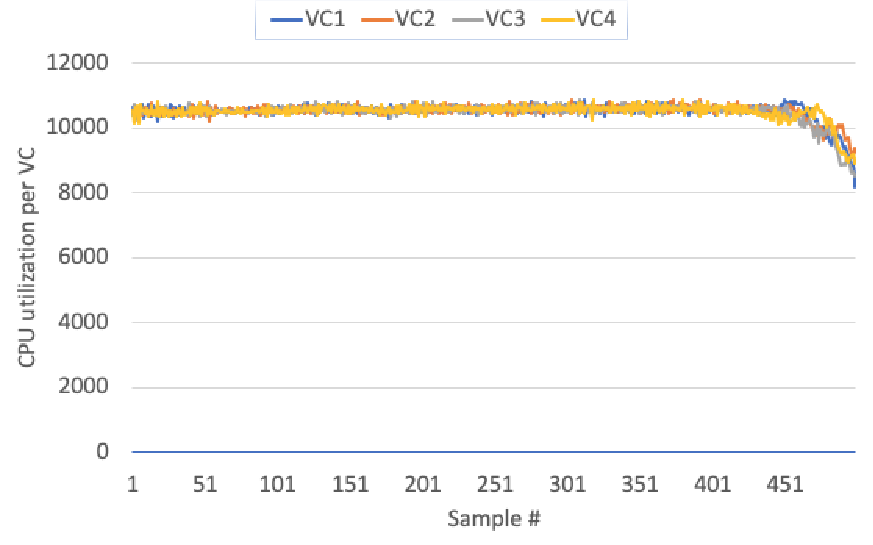
\includegraphics[width=\textwidth]{Figures/per_cluster_utilization_4.pdf}
%          \caption{Running four VCs}
%          %\label{fig:allocation2}
%      \end{subfigure}
%        %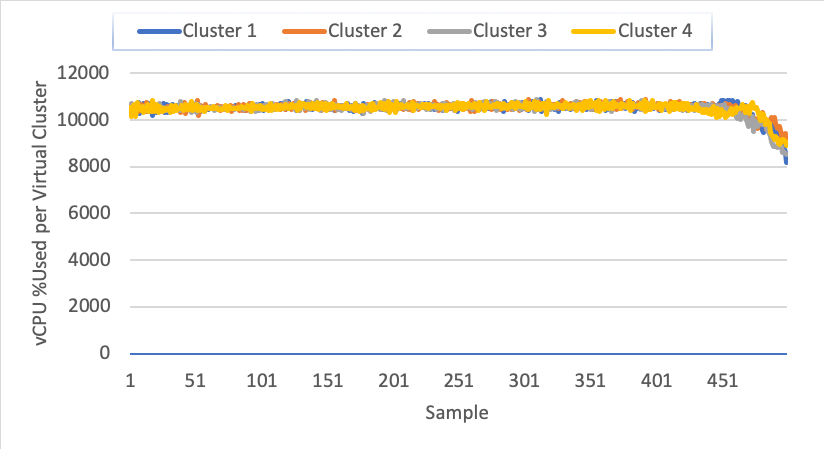
\includegraphics[width=\columnwidth]{Figures/per_cluster_utilization}
%    \end{center}
%    \caption{Plot of CPU utilization per VC at 5-second intervals for fairness check.}
%    \label{fig:per_cluster_utilization}
%    %\vspace{-0.2in}
%  \end{figure}

\subsection{CPU over-commitment with differential QoS}
In addition to the option of equally sharing resources, the proportional, share-based scheduler of the ESXi hypervisor offers a very useful degree of flexibility. This subsection continues the CPU over-commitment study with configuring VCs with different shares, to demonstrate the capability of creating a multi-tenant environment with Quality-of-Service differentiation. 

With the use of CPU shares, each VM can be given a particular guaranteed portion of CPU resources. When there are multiple VMs running on an ESXi host, the ESXi scheduler allocates CPU based on the ratio of shares among all the running VMs. This feature extends to a virtualized HPC cloud. Specifically, each tenant can negotiate an appropriate share of the physical cluster before VC is allocated. In this experiment, we test various shares ratios, and the case of four VCs with 1:1:1:2 shares ratio is shown in Figure~\ref{fig:share_utilization}. Clearly, the CPU utilization ratio among the VCs is the same as the specified shares ratio. %Another important observation is that the aggregate CPU utilization across 4 VCs is the same as the previous equal-shares case as depicted in Figure~\ref{fig:cpu_utilizations}, meaning that the overall system performance is not compromised when shares are customized.


\begin{figure}[!t]
   \begin{center}
       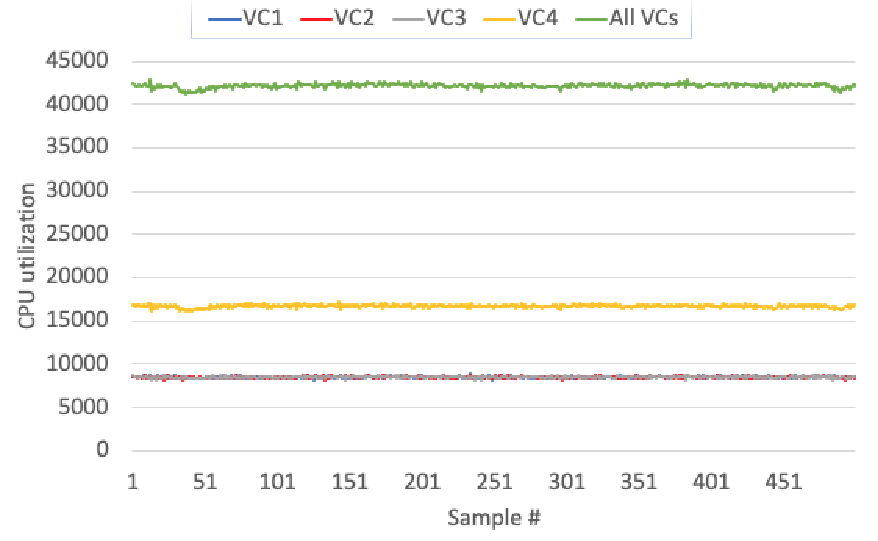
\includegraphics[width=0.8\columnwidth]{Figures/share_utilization.pdf}
   \end{center}
   \caption{CPU utilization for four VCs with 1:1:1:2 CPU shares. Utilization is sampled at 5-second intervals.}
   \label{fig:share_utilization}
 \end{figure}







\subsection{CPU + memory over-commitment}
Given that memory over-commitment is more challenging, 
we only test 2X over-commitment ratio. Specifically, 
we deploy two VCs to achieve 2X over-commitment in both CPU and memory. 
%we only test two VCs with 2X over-commitment in both CPU and memory. 
vSphere Dynamic Resource Scheduler (DRS) is used to control VM migration for load balancing. 
%~\cite{infrastructure2006resource}. 
Considering the VM migration cost, we decide to use four quarter-size VMs per VC on each node, which results in having each tenant own a VC of 32 VMs across the 8-node cluster. 
This is equivalent to using a single full-size VM per VC per node in the sense that each tenant can still access all the physical resources when other tenants are idle. 
%The new configuration is illustrated in Figure~\ref{fig:exp_scenario_2}. 
%As a result, each tenant in this experiment gets a VC of 32 VMs across the 8-node cluster. 

% \begin{figure}[!t]
%    \begin{center}
%        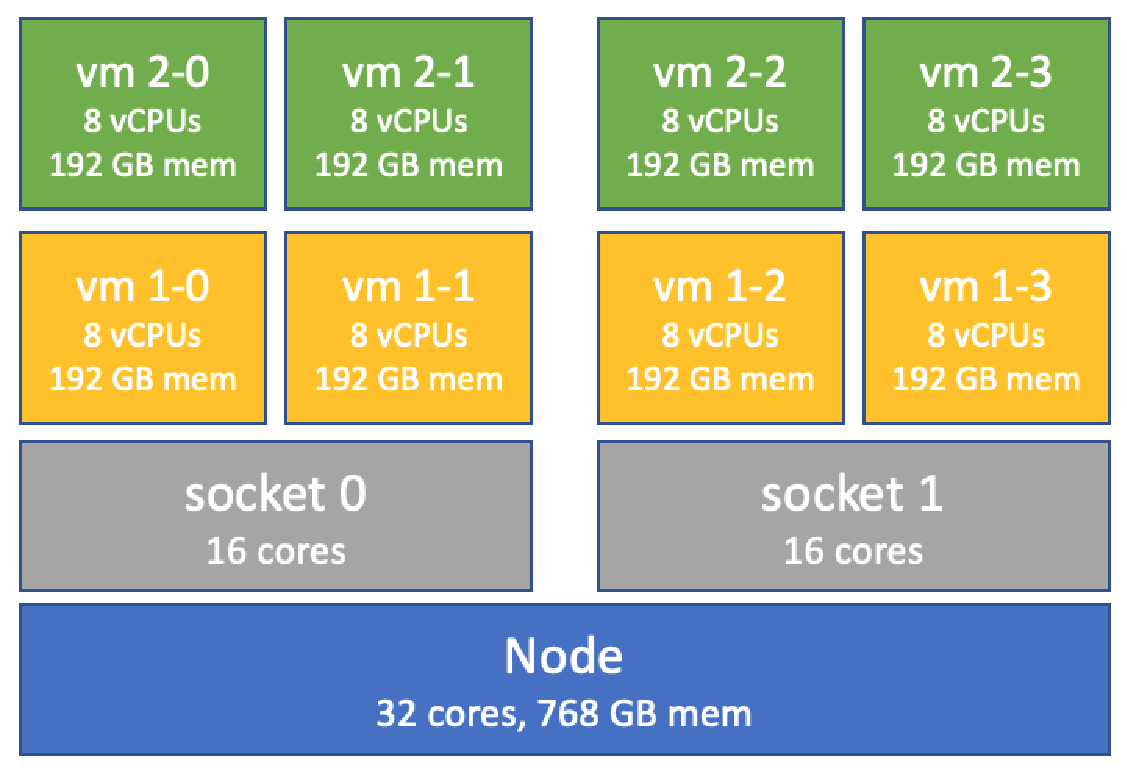
\includegraphics[width=\columnwidth]{Figures/exp_scenario_2.pdf}
%    \end{center}
%    \caption{Illustration of testbed setup for CPU + memory over-commitment experiments. Green VMs and yellow VMs represent two separate VCs.}
%    \label{fig:exp_scenario_2}
%  \end{figure}

To increase memory footprint, we add five HPCC benchmarks (i.e., HPL, RandomAccess, STREAM, PTRANS, and DGEMM). For these  benchmarks, a problem size of 53664 is chosen to have the memory consumption ranging from 16 GB to 22 GB per job instance. All the benchmarks are run with a single threaded process to mimic throughput workloads. 
To model a real HPC tenant, we specify the job arrival time to follow a Gamma distribution based on an study of several production HPC systems~\cite{lublin2003workload}.  
%The resulting mean job inter-arrival time is 20.88 seconds
The Gamma distribution has a shape parameter of 10.23 and scale parameter of 0.49, which means the mean job inter-arrival time is 10.23 / 0.49 = 20.88 seconds. 
Also, all job sequences are shuffled to generate randomized job streams. %Then, two execution scenarios are designed to represent different workload patterns. 

Three execution scenarios are designed to represent different workload patterns. 
Table~\ref{tbl:scenarios} lists the details of each scenario and emphasizes on the differences.
Note that due to the varying memory consumption of the different HPCC benchmarks coupled with the stochastic behavior of the job arrivals, we cannot calculate the memory load in GB but instead classify the load into either heavy or light.  

\begin{table*}[!h]\small
  \caption{CPU + memory over-commitment experiment scenarios.}
  \centering
    \begin{tabular}{|l|c|c|c|c|c|c|}
    \hline
    Scenario & \multicolumn{2}{|c|}{Scenario 1} & \multicolumn{2}{|c|}{Scenario 2} & \multicolumn{2}{|c|}{Scenario 3} \\
    \hline
    Cluster & VC1 & VC2 & VC1 & VC2 & VC1 & VC2 \\
    \hline
    \#jobs & 1500 & 1500 & 1600 & 1500 & 1600 & 1600 \\
    \hline
    Workloads & BioPerf & BioPerf & HPCC & BioPerf & HPCC & HPCC \\
    \hline
    \multirow{2}{*}{Job arrival} & \multirow{2}{*}{stochastic} & \multirow{2}{*}{stochastic} & deterministic, all enqueued & \multirow{2}{*}{stochastic} & \multirow{2}{*}{stochastic} & \multirow{2}{*}{stochastic} \\
                                & &  & at the same time & & & \\
    \hline
    CPU load & heavy & heavy & heavy & heavy & heavy & heavy\\
    \hline
    Memory load & light & light & heavy & light & heavy & heavy \\
    \hline
    \end{tabular}
  \label{tbl:scenarios}
\end{table*}

In the first scenario, both VCs stochastically launch 1500 BioPerf jobs following the above Gamma 
distribution. Since BioPerf benchmarks are CPU-intensive and memory-light, the purpose of this 
experiment is to test the feasibility of provisioning memory with over-commitment while not actively over-stressing the memory. 

In the second scenario, 1600 memory-intensive HPCC jobs are enqueued to the first VC immediately after the experiment begins, while 1500 BioPerf jobs stochastically arrive at the second VC following the above Gamma distribution. The number of jobs are selected to let the two VCs finish at roughly the same time. In the first VC, all the job slots will be consumed
immediately and the jobs will maximize their utilization of the cluster's CPU and memory resources. In the second cluster, CPU and memory load will gradually build up as more jobs arrive. 
%This experiment scenario is summarized in Table~\ref{tbl:scenario1}. 




% \begin{table}[!h]\small
%   \caption{CPU + memory over-commitment, Scenario 1.}
%   \centering
%     \begin{tabular}{|c|c|c|}
%     \hline
%      & VC1 & VC2 \\
%     \hline
%     \#jobs & 1600 & 1500 \\
%     \hline
%     Workloads & HPCC & BioPerf \\
%     \hline
%     Job arrival & deterministic, all enqueued & stochastic \\
%     & at the same time & \\
%     \hline
%     CPU load & heavy & heavy \\
%     \hline
%     Memory load & heavy & light \\
%     \hline
%     \end{tabular}
%   \label{tbl:scenario1}
% \end{table}

The third scenario is designed to be the most demanding by running two HPCC streams each following the Gamma distribution. 
%Were all job slots being used, the active memory consumption would largely exceed the physical memory capacity. 
Even if each job only consumes 16 GB memory (i.e., the minimum among the HPCC benchmarks), 64 job instances on each node will require 64 * 16 GB = 1024 GB, which is much larger than the node memory capacity of 768 GB. It is obvious that ESXi cannot support that level of memory over-usage. But, it is still worthwhile to explore in the realistic case where jobs randomly come and go, whether DRS can collaborate with ESXi memory reclamation to accommodate this usage pattern. 

% \begin{table}[!h]\small
%   \caption{CPU + memory over-commitment, Scenario 2.}
%   \centering
%     \begin{tabular}{|c|c|c|}
%     \hline
%      & VC1 & VC2 \\
%     \hline
%     \#jobs & 1600 & 1600 \\
%     \hline
%     Workloads & HPCC & HPCC \\
%     \hline
%     Job arrival & stochastic & stochastic \\
%     \hline
%     CPU load & heavy & heavy \\
%     \hline
%     Memory load & heavy & heavy \\
%     \hline
%     \end{tabular}
%   \label{tbl:scenario2}
% \end{table}

In each scenario, we run with and without DRS and measure two metrics: 1) wall clock time (WCT), i.e., the elapsed time from the start of job submission to the completion of the last job; 2) cumulative job execution time (CJET), i.e., the cumulative sum of all job instances' execution time. We don't compare to bare-metal as a second boot disk is not available on this testbed. 

The results in scenario 1 are plotted in Figure~\ref{fig:memory_scenario_1}. 
Both VCs are able to complete the entire job sequence, demonstrating the success of 
provisioning multiple VCs with CPU and memory over-commitment. 
Figure~\ref{fig:memory_scenario_1} shows that the two 
VCs have the same WCT and CJET. This again confirms that fairness is maintained even 
under resource over-commitment. The WCT difference between DRS enabled and DRS disabled 
is negligible because WCT is dominated by the stochastic job arrival. That is, 
even if previous jobs finish earlier, the last job's arrival time is specified 
by the Gamma distribution beforehand. 
However, CJET in 
Figure~\ref{fig:memory_cjet_1} is able to reveal the benefits of DRS: the time spent on executing jobs is reduced by 29.6\% in both VCs, 
making room available for accommodating more jobs in the system. The number of VM migrations 
is around 50 during each 10-hour run. 

\begin{figure}
     \centering
     \begin{subfigure}[b]{0.4\textwidth}
         \centering
         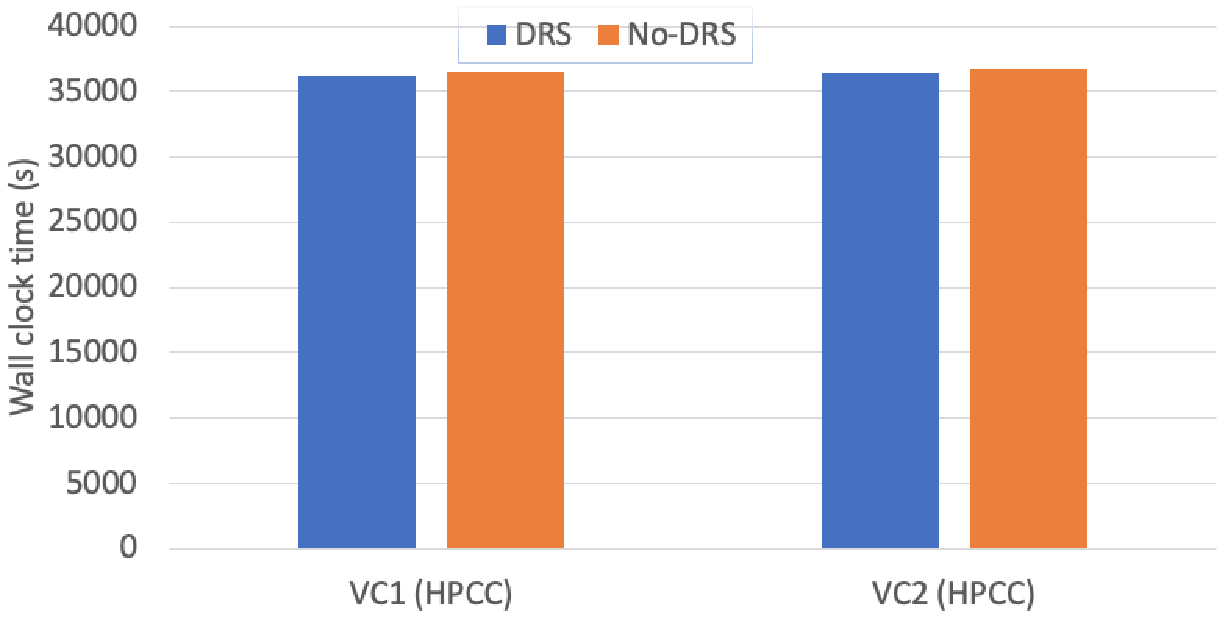
\includegraphics[width=\textwidth]{Figures/memory_wct_1.pdf}
         \caption{Wall clock time}
         \label{fig:memory_wct_1}
     \end{subfigure}
     \hfill
     \begin{subfigure}[b]{0.4\textwidth}
         \centering
         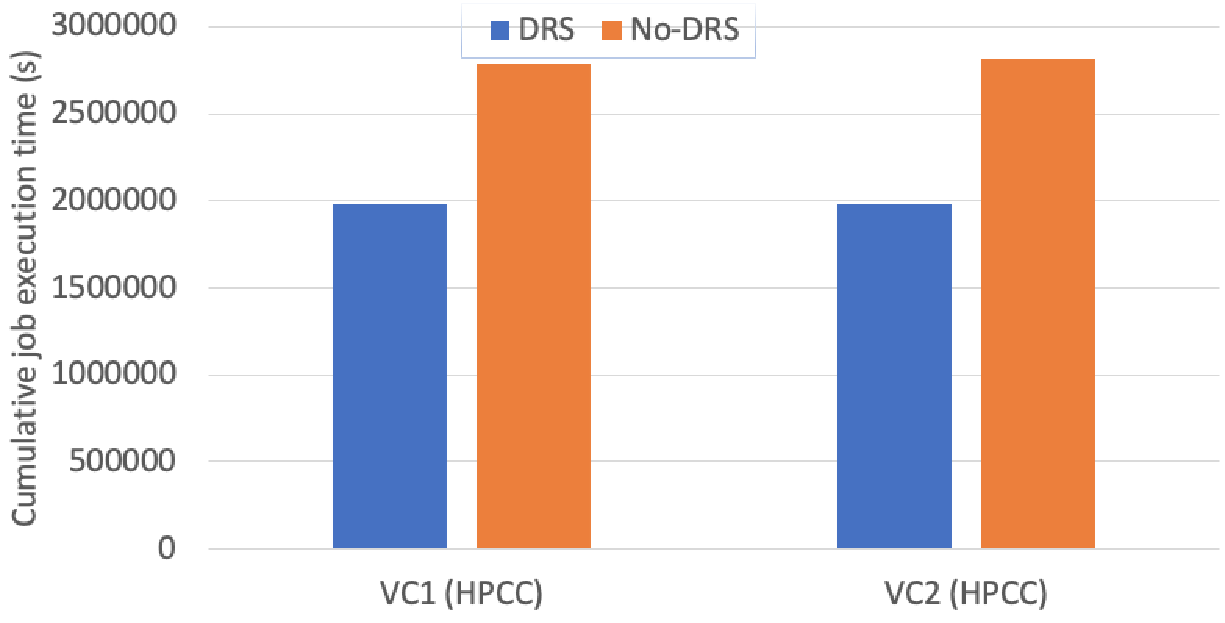
\includegraphics[width=\textwidth]{Figures/memory_cjet_1.pdf}
         \caption{Cumulative job execution time}
         \label{fig:memory_cjet_1}
     \end{subfigure}
     \caption{Comparison between DRS enabled and DRS disabled for 2X CPU and memory over-commitment. Workloads are from scenario 1. }
     \label{fig:memory_scenario_1}
\end{figure}

%The first metric is a measure of the system throughput, and the second metric indicates system efficiency. 
Figure~\ref{fig:memory_scenario_2} shows the results in scenario 2. As the graphs suggest, while VCs successfully supports 2X CPU and memory over-commitment regardless of DRS, DRS reduces HPCC's WCT by 11.1\%, which is a great improvement in throughput. 
Similar to scenario 1, the reason why DRS doesn't reduce BioPerf's WCT is that BioPerf jobs strictly follow the Gamma distribution in job arrivals.
But as we can see in Figure~\ref{fig:memory_cjet_2}, DRS reduces BioPerf's CJET by 18.4\%.
%, making room available for accommodating more jobs in the cluster. 
HPCC's CJET slightly increases with DRS and it indicates that DRS can incur some overhead 
due to telemetry sampling and VM migration. 
%, but increases HPCC CJET by 1.1\%, which is negligible. 
The number of VM migrations in each run is in the range of 30-40. It's interesting to notice that all migrations happened to the BioPerf VMs, because BioPerf VMs have smaller memory footprint and are thus cheaper to migrate.

\begin{figure}
     \centering
     \begin{subfigure}[b]{0.4\textwidth}
         \centering
         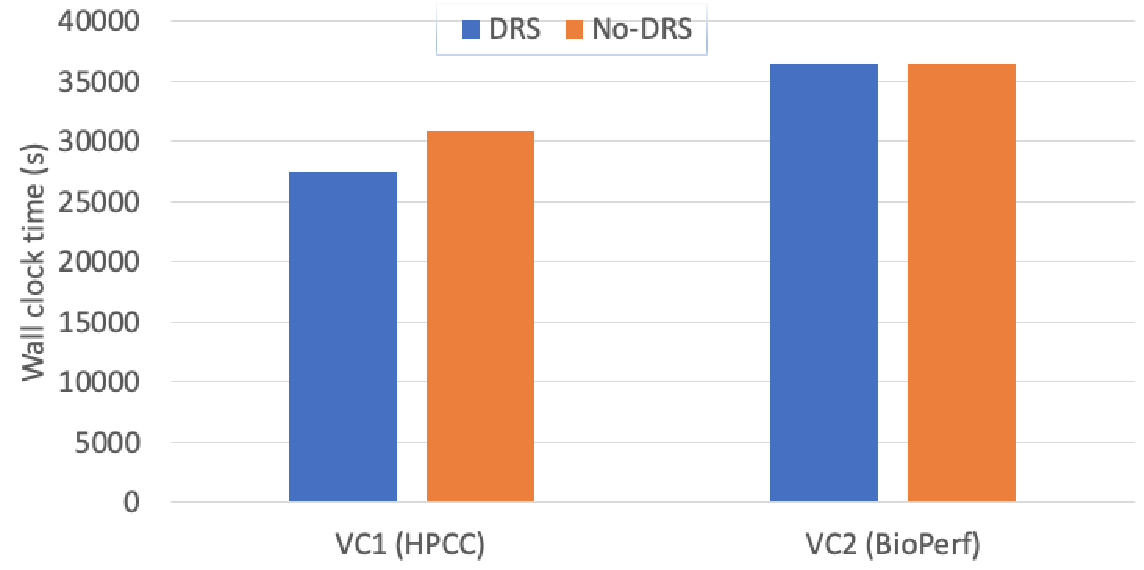
\includegraphics[width=\textwidth]{Figures/memory_wct_2.pdf}
         \caption{Wall clock time}
         \label{fig:memory_wct_2}
     \end{subfigure}
     \hfill
     \begin{subfigure}[b]{0.4\textwidth}
         \centering
         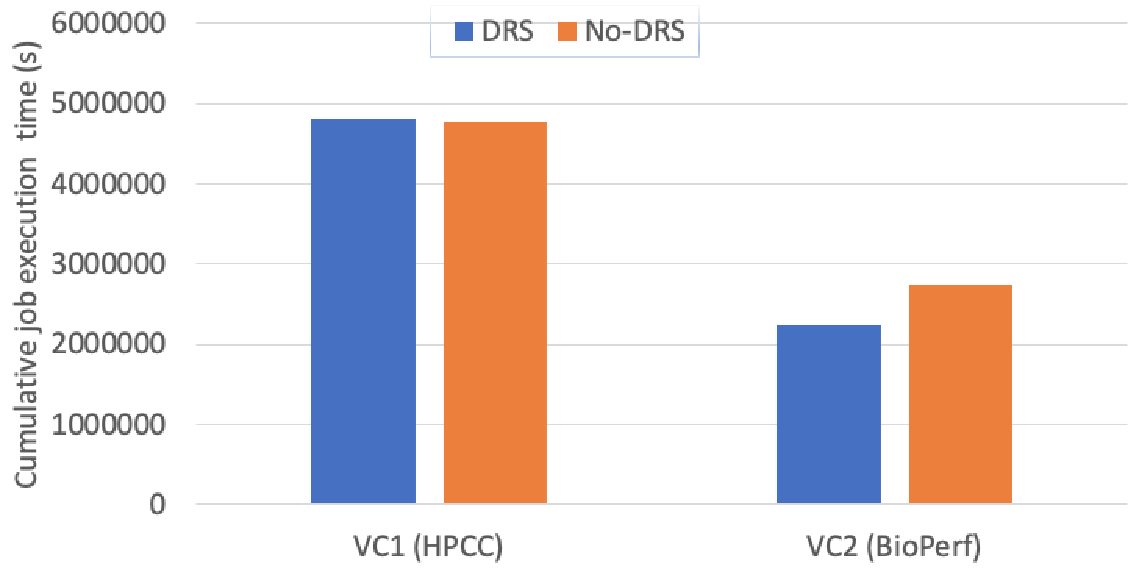
\includegraphics[width=\textwidth]{Figures/memory_cjet_2.pdf}
         \caption{Cumulative job execution time}
         \label{fig:memory_cjet_2}
     \end{subfigure}
     \caption{Comparison between DRS enabled and DRS disabled for 2X CPU and memory over-commitment. Workloads are from scenario 2. }
     \label{fig:memory_scenario_2}
\end{figure}

As explained above, the third scenario is much more demanding because HPCC jobs can potentially consume all the over-committed VM memory. It's not a surprise that the system under test is not able to finish two simultaneous streams of HPCC jobs, regardless of whether DRS is used or not. Specifically, some guest OSes encounter CPU soft lockup errors and hang before they finish the job stream. Our investigation identifies that the problem appears when hypervisor starts to swap memory to disk and becomes unresponsive to guest OS memory demands. Since hypervisor swapping 
is triggered by the free memory reaching a per-host threshold, this problem is avoidable by carefully calibrating the co-located workloads to not exceed the threshold~\cite{banerjee2013memory}. For example, an SLA (service-level agreement) term can be defined to confine a tenant's memory usage in certain time periods. 

Our analysis further identify HPL benchmark as the bottleneck. Each HPL job needs more than 3 hours to finish, and once enough HPL instances accumulate on any node, the hypervisor is not able to handle their excessive memory requirements. After removing HPL from the benchmark suite, we see that two HPCC streams can finish when DRS is enabled. Without DRS, the same failure occurs. Clearly, this demonstrates that DRS can assist ESXi memory reclamation techniques in achieving higher level of memory over-commitment. 

Though HPCC VMs are heavy to migrate, on average 67 VM migrations occurred per run, due to the extreme memory stress. Naturally, one may be concerned that the large number of migrations could introduce jitters to the running workloads. To quantify that, we collect the execution time distribution among all job instances of each benchmark. It turns out that the execution time, even in the case of memory over-commitment, maintains good consistency. For example, the histograms of RandomAccess and DGEMM are shown in Figure~\ref{fig:histogram}, and the histogram graphs of STREAM and PTRANS are similar to those of RandomAccess and DGEMM. It can be seen that most job instances fall into the first two bins in both Figure~\ref{fig:ra_histogram} and Figure~\ref{fig:dgemm_histogram}. At the same time, due to memory reclamation and VM migration, some job instances experience non-negligible delays and fall outside of the first two bins as expected. However, the percentage of such instances are all below 1\% for all benchmarks. Given that these HPCC benchmarks represent memory-intensive HPC workloads, these results demonstrate that our approach can achieve two 9s tail latency guarantee at 2X CPU + memory over-commitment. 


\begin{figure}
     \centering
     \begin{subfigure}[b]{0.4\textwidth}
         \centering
         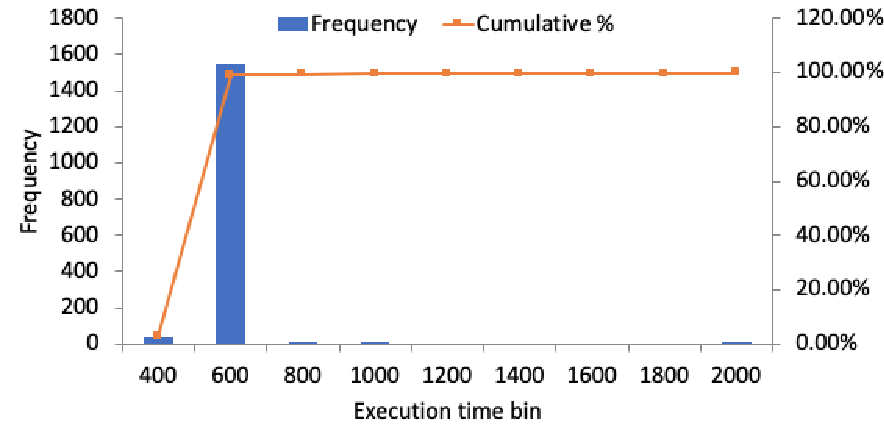
\includegraphics[width=\textwidth]{Figures/ra_histogram.pdf}
         \caption{RandomAccess}
         \label{fig:ra_histogram}
     \end{subfigure}
     \hfill
     \begin{subfigure}[b]{0.4\textwidth}
         \centering
         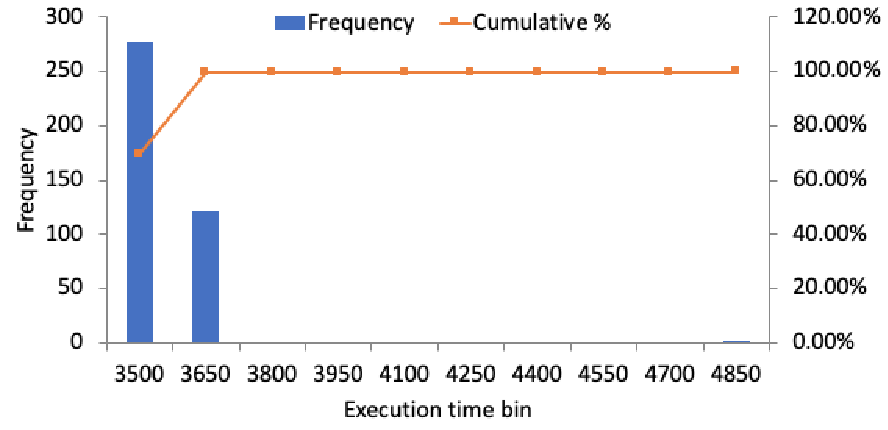
\includegraphics[width=\textwidth]{Figures/dgemm_histogram.pdf}
         \caption{DGEMM}
         \label{fig:dgemm_histogram}
     \end{subfigure}
     \caption{Histogram of individual job execution time from both VCs. Left X-axis is frequency and right X-axis is cumulative percentage.}
     \label{fig:histogram}
\end{figure}
% \begin{figure}[!t]
%    \begin{center}
%        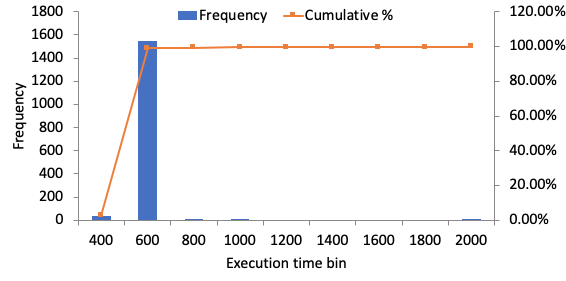
\includegraphics[width=\columnwidth]{Figures/ra_histogram}
%    \end{center}
%    \caption{Histogram of individual RandomAccess job execution time from both VCs.}
%    \label{fig:ra_histogram}
% \end{figure}




